\chapter{Testbed - Prototype Implementation}
\label{chap:referenceimplementation}

As already discussed in Chapter \ref{chap:introduction}, sensing a city's parking availability and thus making the parking situation more transparent would be highly beneficial for reducing traffic congestion and greenhouse gas emissions as driver's looking for parking spaces in urban areas could navigate directly to vacant parking spaces close to their destinations. To support this goal, a prototype of drive-by sensing using an optical distance sensor has been designed, implemented, and evaluated. This chapter introduces the prototype and testbed which have been developed to acquire the necessary dataset to run the machine learning experiments. First, the used hardware and sensors are described (Section \ref{sec:test_bed}), then the software to collect test data is being discussed (Section \ref{sec:sensor_measurement_collection}) and finally the acquired raw sensor dataset is shown (Section \ref{sec:raw_dataset}).





\section{Used Hardware and Sensor Parts}
\label{sec:test_bed}

Figure \ref{fig:sensing_car} shows the sensing car and its mounted sensors. For collecting, processing, and saving the sensed data a Raspberry Pi 2 Model B\footnote{\url{https://www.raspberrypi.org/products/raspberry-pi-2-model-b/}} is used. A Raspberry Pi was chosen because of its simplicity to connect and access sensors and moreover because it is really easy to program as it is just a regular Linux-based computer. Furthermore, the price of a Raspberry Pi is also quite low (about \euro{35}), therefore the overall cost of the system will remain low.


\begin{figure}
	\centering
	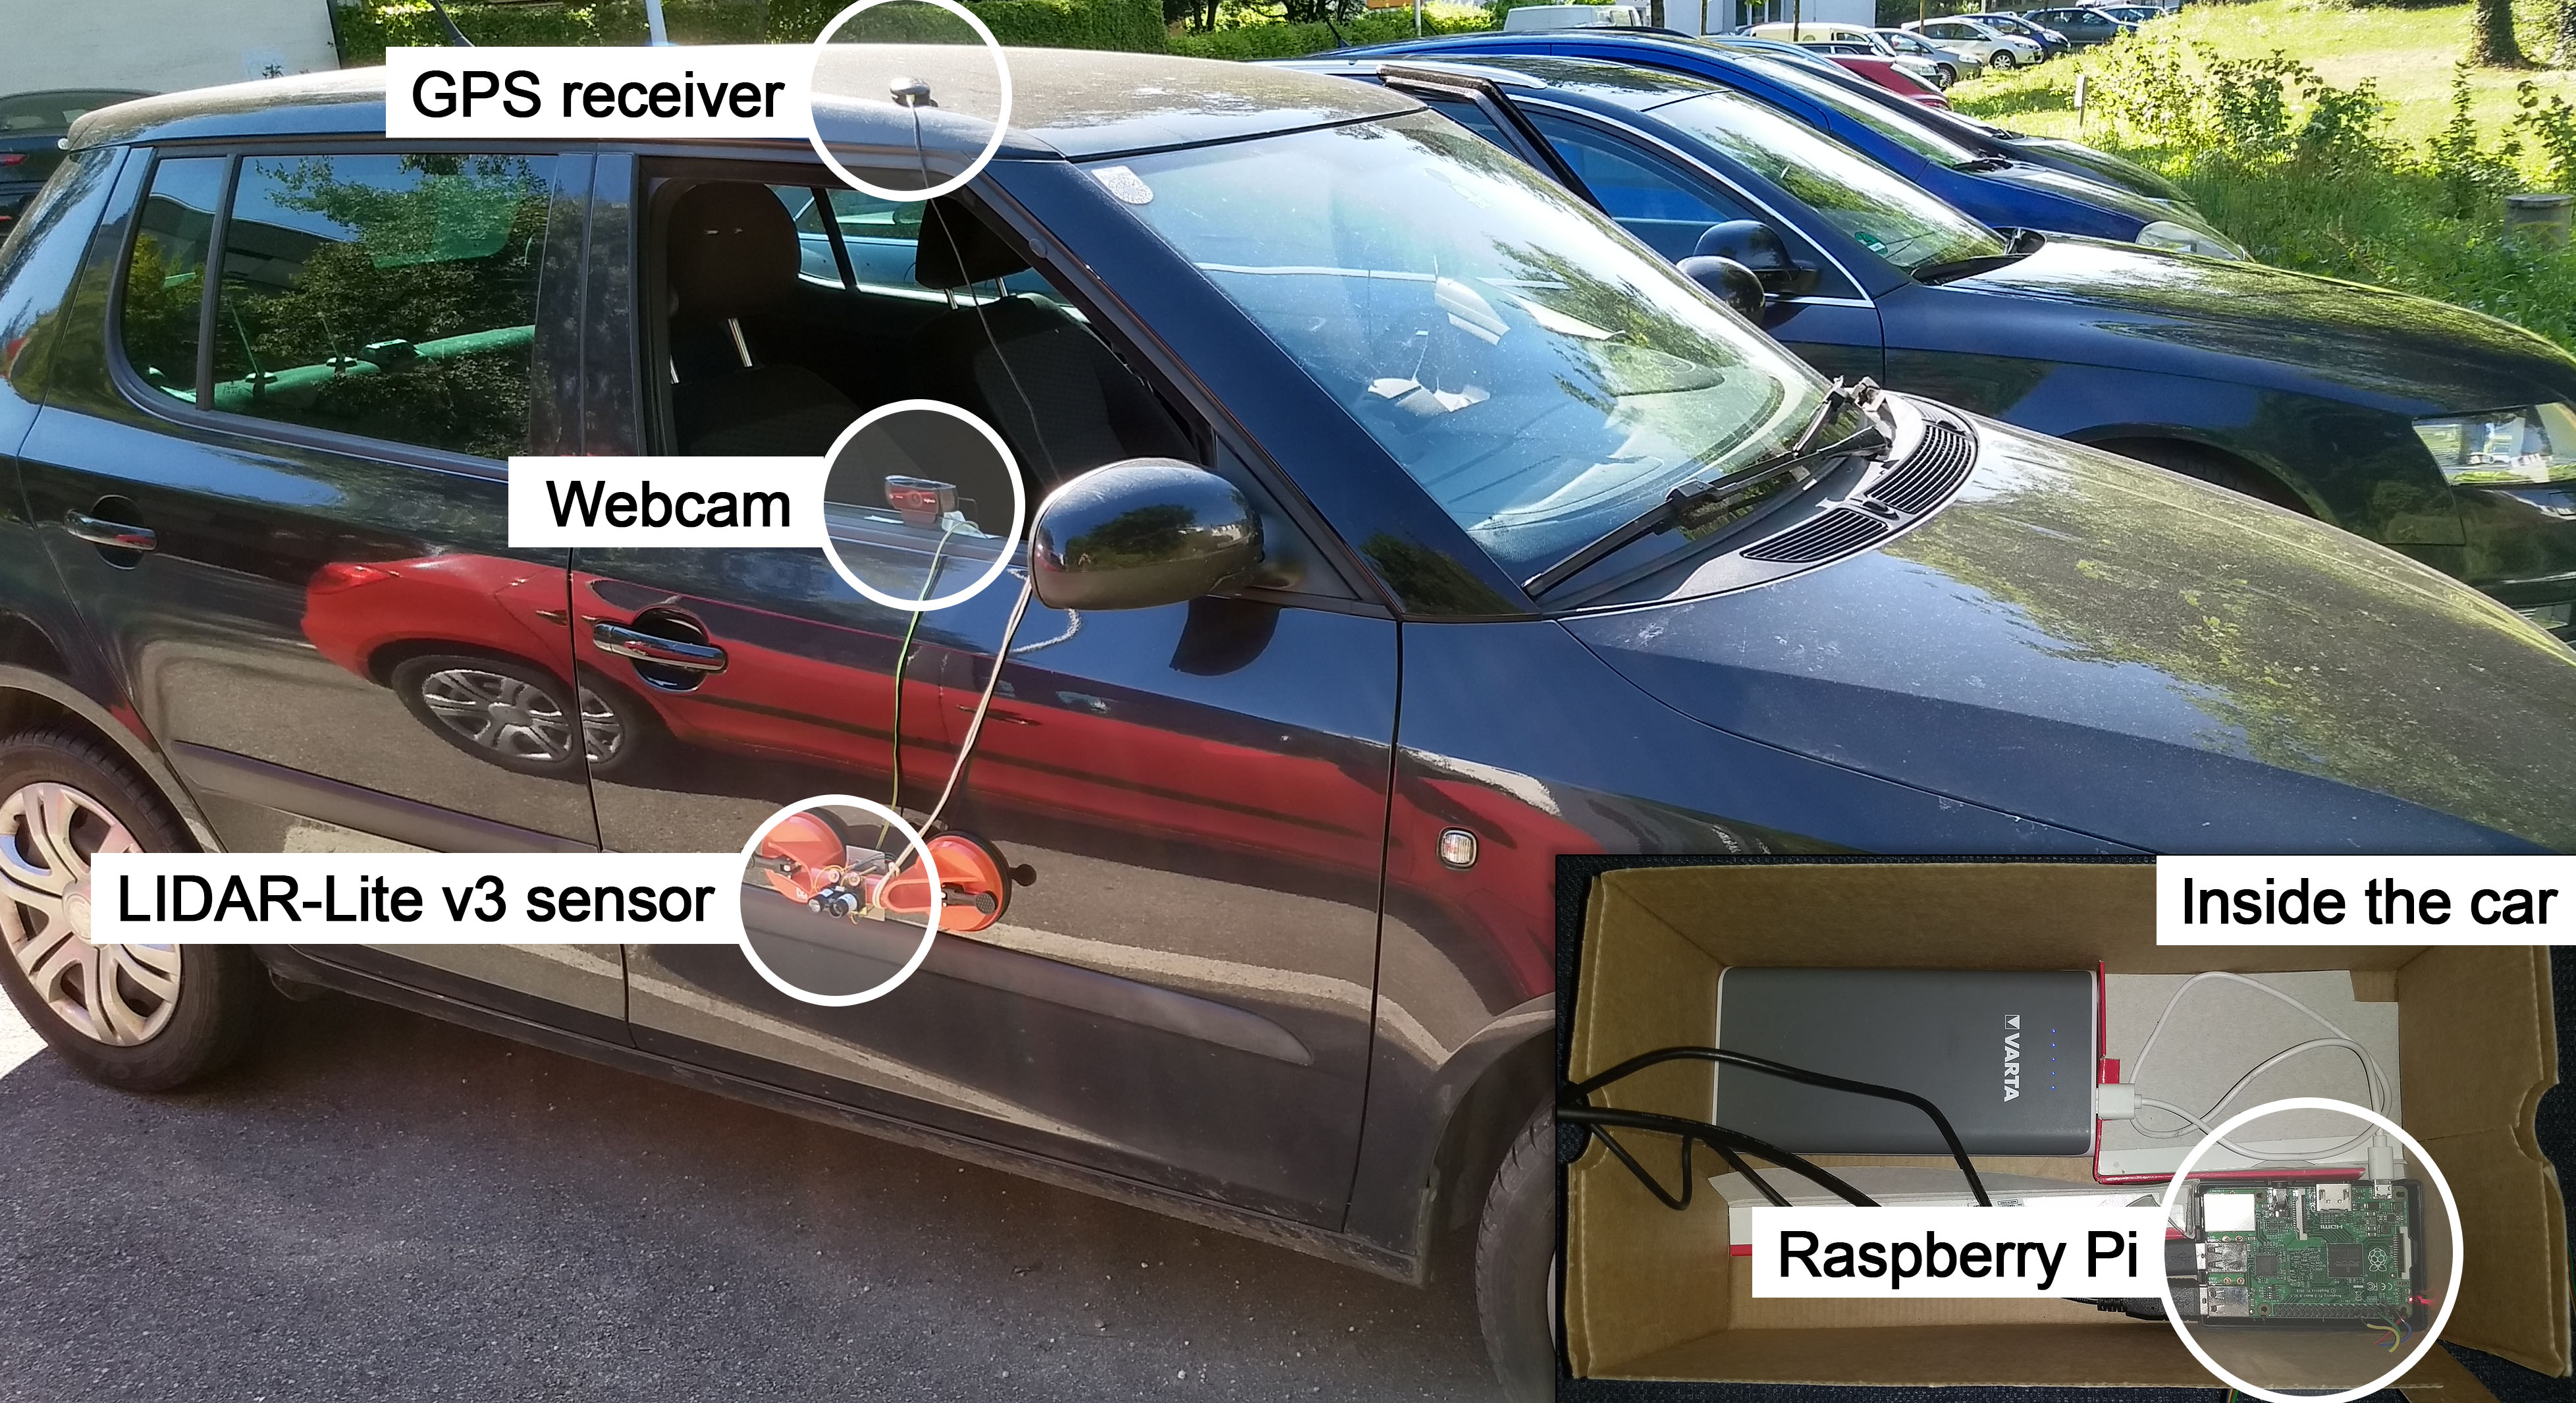
\includegraphics[width=0.8\textwidth]{img/car.jpg}
	\caption{Prototype of the sensing car, which is composed of a LIDAR Lite v3 optical distance sensor, a GPS receiver, a camera for ground truth collection and a Raspberry Pi as processing device.}
	\label{fig:sensing_car}
\end{figure}


To determine the location of the sensing vehicles while driving through the city, a Navilock USB GPS receiver\footnote{\url{http://www.navilock.de/produkte/G_61840/merkmale.html?setLanguage=en}} is used. The receiver is connected to the Raspberry Pi using a USB port and measures the GPS location (latitude and longitude) at a rate of about 1 Hz. According to the manufacturer the acquired positions are correct in the range of 2.5 meters. The GPS receiver is mounted on the top of the sensing car using a magnet in order to receive more accurate sensor readings. The Navilock USB GPS sensor costs about \euro{50}.

Two major distance sensor technologies can be differentiated: an ultrasonic range sensor and an optical laser distance sensor. While ultrasonic sensors are cheap and widely used in commercial parking assistance systems, they also have limitations in terms of sensing frequency (about 20 Hz) and range (a few meters). These specifications limit the use of ultrasonic sensors for drive-by sensing on multi-lane roads or high speed. Due to these limitations an optical distance sensor, the "Lidar Lite v3\footnote{\url{https://www.sparkfun.com/products/14032}}" is used in our testbed. It measures the time of flight of an emitted laser signal which is reflected by an object in its way. The Lidar Lite v3 can measure distances from a few centimeters up to 40 meters at a frequency of 1 to 500 Hz. Furthermore, it is able to measure distances with an accuracy of about 2.5 centimeters. However, in comparison to ultrasonic sensors, optical sensors are more expensive. While the costs of ultrasonic sensors are often below \euro{10}, the Lidar Lite v3 and other comparable sensors cost about \euro{150}.

The distance sensor is mounted on the co-driver's door using a sucker handle in order to face the right side of the road and to take measures at about 62 cm above the ground. It is connected to the Raspberry Pi via GPIO (General Purpose Input Output) pins, communicating using an I2C (Inter Integrated Circuit) interface, according to the manufacturer's specifications.

Table \ref{table:comparison_us_lidar} shows a comparison of the characteristics of ultrasonic sensors and the Lidar Lite v3 sensor. The most significant limitation is the sampling frequency. While optical laser sensors are based on the speed of light, ultrasonic sensors are based on the speed of sound, which is much lower. Therefore, also the distance between consecutive measurements varies highly from an ultrasonic to an optical laser sensor. At a speed of 50 km/h, the distance between two consecutive measurements is up to 70 cm using an ultrasonic sensor while it is only about 3 cm when using an optical distance sensor.



\begin{table}


\resizebox{\textwidth}{!}{%
\bgroup
\def\arraystretch{1.4}
\begin{tabular}{| r || c | c |}
\hline
   & 
   \textbf{Ultrasonic Range Finder} & 
   \textbf{Lidar Lite v3} \\
%\hline
\hline
  \textbf{Costs} & 
   from about \euro{5,00} to \euro{100,00} &
   about \euro{150,00} \\
\hline
  \textbf{Sampling Frequency} & 
   up to 20 Hz &
   up to 500 Hz \\
   & (at 10 m distance) & \\
\hline
  \textbf{Range} & 
   2 cm - 10 m &
   30 cm - 40 m \\
\hline
  \textbf{Distance between Measurements} & 
   about 70 cm &
   about 3 cm \\
  \textbf{at 50 km/h} & & \\
\hline

\end{tabular}
\egroup
}

\caption{Comparison of ultrasonic sensors and the used Lidar Lite v3 optical distance sensor.}
\label{table:comparison_us_lidar}
\end{table}

A camera is leveraged to capture images of the ground truth, here, a Logitech C922 Pro Stream\footnote{\url{https://www.logitech.com/en-us/product/c922-pro-stream-webcam}} is used. Images with a resolution of 352 x 288 pixels are captured at a frequency of about 30 Hz while the car is sensing parking spaces. The camera is mounted on the co-driver's door on the same horizontal position as the sensor. This way the center of the image will be the position where the distance measurement is taken. The Logitech camera is connected to the Raspberry Pi using an USB port and is available at about \euro{90}.





%\begin{table}
%
%\bgroup
%\def\arraystretch{1.5}
%\begin{tabular}{| r || c | c |}
%\hline
%   & 
%   \textbf{Sampling Frequency} & 
%   \textbf{Costs per Sensor} \\
%%\hline
%\hline
%  \textbf{Lidar Lite v3} & 
%   ~200 measurements/s &
%   \euro{169,00} \\
%\hline
%  \textbf{Navilock USB} & 
%   ~1 measurement/s &
%   \euro{74,90} \\
%   \textbf{GPS receiver} & & \\
%\hline
%
%\end{tabular}
%\egroup
%
%\caption{The used sensors}
%\label{table:sensors_capabilities}
%\end{table}


\section{Collecting Sensor Measurement Data}
\label{sec:sensor_measurement_collection}

A Python script has been developed which saves all sensor readings during the test runs into a text file for later analysis and evaluation. Furthermore, all images captured by the camera are saved into a specific folder on the Raspberry Pi to be able to derive the ground truth information later on (see Section \ref{sec:ground_truth_tagging}).
The sensing of all three devices (GPS, Lidar Lite v3, Logitech camera) is performed asynchronously in separate threads so that none of them influence the other sensor's readings. For accessing the GPS receiver the Python GPS library is used whereas for measuring the distance using the Lidar Lite v3 sensor, an open source library available on github.com is used\footnote{\url{https://github.com/Sanderi44/Lidar-Lite}}. 
%A library called "pygame.camera" was used to capture the images of the webcam. 

Figure \ref{fig:sample_sensor_trace} shows how the sensor data gets collected and furthermore presents a sample of raw sensor data derived during a test drive. The sensor data text file contains GPS and distance measurements. The first column contains the sensor type. The second column gives the time stamp of the Raspberry Pi's system time in seconds. GPS measurements also result in latitude, longitude and speed values while the Lidar Lite measurements result in the measured distance in centimeters.

%\begin{figure}
%	\centering
%	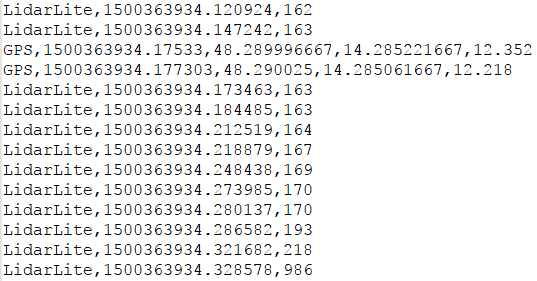
\includegraphics{img/sample-sensor-trace.PNG}
%	\caption{Sample of the collected sensor trace}
%	\label{fig:sample_sensor_trace}
%\end{figure}

\begin{figure}
	\centering
	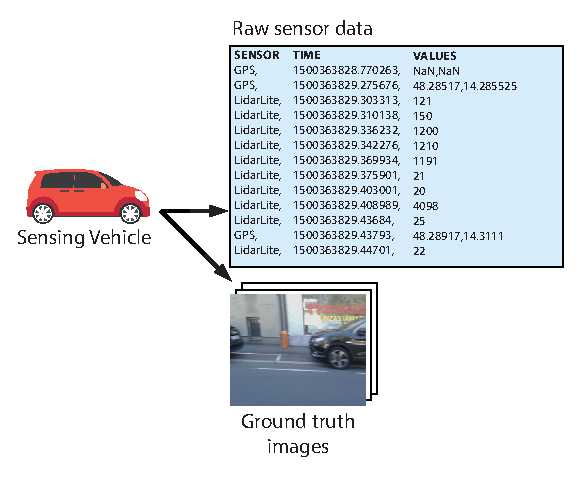
\includegraphics{img/obtaining-raw-dataset.eps}
	\caption{Acquiring raw sensor data.}
	\label{fig:sample_sensor_trace}
\end{figure}



\section{Raw Data Set}
\label{sec:raw_dataset}

To obtain a dataset, in total 32 test drives were completed in the city of Linz, Austria. The street scenarios have been selected aiming at a high variability of road scenarios. The test scenes include single lane as well as multi lane streets. While collecting the test measurements the sensing car was driving as it would in regular traffic (not only in the right most lane, etc.) and the scenes also include high and low traffic scenarios. For all street scenarios, measurements have been repeated multiple times.
Figure \ref{fig:gps_locations_dataset} shows an aggregated GPS trace of all test drives on a map of Linz. Red dots represent parking cars while black dots represent other objects. In total \textbf{444.427 distance measurements} and \textbf{14.997 GPS measurements} were taken, which makes up about 15,9 megabytes of distance and GPS data. 
Additionally, \textbf{266.309 images} were captured to record the ground truth of the sensed scenes. The images, which make up about \textbf{5.072 megabytes}, are used to determine the ground truth of the recorded scenes. Sensed data and ground truth data are applied to supervised machine learning algorithms later on. Ground truth tagging is described in the following section.



\begin{figure}
	\centering
	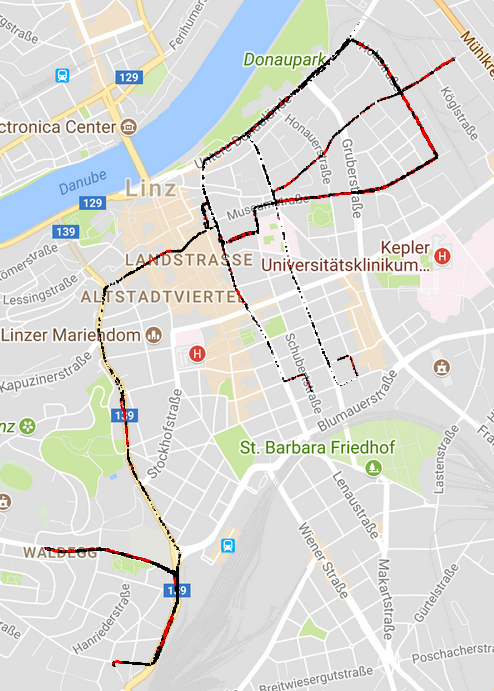
\includegraphics{img/gps_data_recorded_data_parking_spaces.PNG}
	\caption{GPS trace of all recorded samples in the acquired dataset, while 32 test drives in Linz, Austria. Red dots represent parking cars.}
	\label{fig:gps_locations_dataset}
\end{figure}


















\chapter{Data Processing and Machine Learning Approaches}
\label{chap:data_processing_and_ml}

This chapter describes all the steps which are necessary to prepare the raw dataset for the use in machine learning. The required steps include manual ground truth tagging (Section \ref{sec:ground_truth_tagging}), data preprocessing (Section \ref{sec:data_preprocessing}), data segmentation (Section \ref{sec:data_segmentation}), and feature calculation (Section \ref{sec:feature_calculation}).
Furthermore, the use of parking space maps is being discussed to possibly improve the dataset and also the classification results (Section \ref{sec:parking_space_maps}). The derived datasets are described in Section \ref{sec:derived_dataset}, providing an analysis of the datasets and the features. Finally, the machine learning- and deep learning experiments (Sections \ref{sec:machine_learning_experiments} and \ref{sec:deep_learning}) are discussed including the used machine learning models, used tools and the evaluation process.





\section{Ground Truth Tagging}
\label{sec:ground_truth_tagging}

The recorded raw dataset contains distance and position measurements as well as images showing the ground truth at a specific point in time. To be able to process the ground truth information included in the images, a manual ground truth tagging task has to be performed. Figure \ref{fig:ground_truth_tagging_ui} shows the user interface of the program which has been implemented to manually tag an image with one of nine pre selected class labels. The file name of each image is the time stamp of the recording. After the images are loaded, the user has to tag the situation which is present at the center of the image (red line). For instance, Figure \ref{fig:ground_truth_tagging_ui} shows a parking car at the center of the image. In addition, on the right side of the image, a car which has been overtaken by the sensing vehicle is also visible, but as it is not in the center, the image is labelled as "parking car".
Possible class labels are: 

\begin{figure}
	\centering
	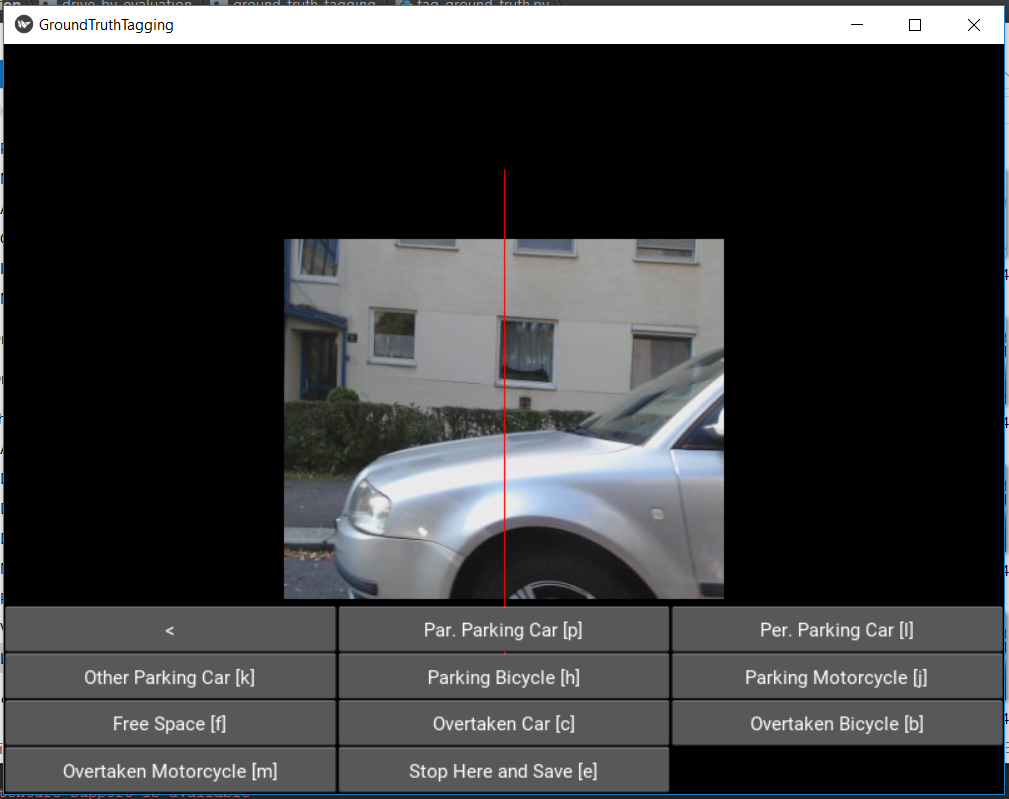
\includegraphics[width=0.85\textwidth]{img/ground_truth_tagging_ui.PNG}
	\caption{User interface for manual tagging of parking situations. \todo{crop}}
	\label{fig:ground_truth_tagging_ui}
\end{figure}

\begin{description}

\item[Parking car:] A parking car is a non-moving vehicle which is parking at the right side of the road. There are three kinds of parking vehicles: \textbf{\textit{Parallel parking cars}}, \textbf{\textit{perpendicular parking cars}}, and \textbf{\textit{angular parking cars}}. Figure \ref{fig:types_of_parking_cars} shows the different types of parking spaces.

\item[Overtaking situation:] This class label means that the sensing vehicle is overtaking another road vehicle. The user can choose between \textbf{\textit{overtaken cars}}, \textbf{\textit{overtaken motorcycles}} and \textbf{\textit{overtaken bicycles}}.

\item[Other parking vehicle:] The user can also tag \textbf{\textit{parking motorcycles}} and \textbf{\textit{parking bicycles}}. This class represents obstacles which can be located on parking spaces and therefore make it unavailable for parking.

\item[Free space:] This class label should be used, when none of the above listed class labels are applicable. It represents a free space where it is maybe possible to park a vehicle. Yet only with the help of a parking space map, a free space can be marked as vacant parking space as a random free space may be an illegal parking space (e.g. a driveway).

\end{description}



The output of the ground truth tagging process is persistently saved as a text file where each line contains an entry with a time stamp and its corresponding tagged ground truth class label. This ground truth file will be further processed during the machine learning process as described in \todo{ref}.


\begin{figure}
	\centering
	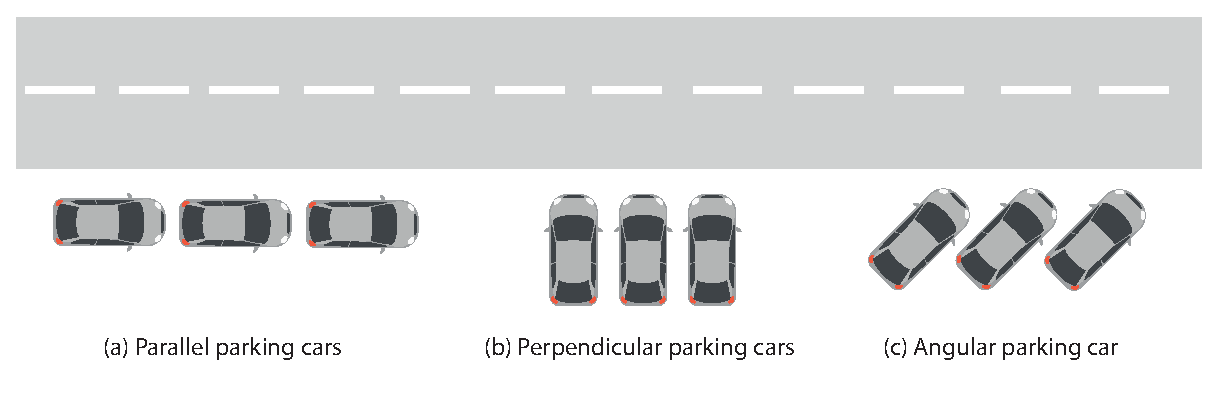
\includegraphics[width=\textwidth]{img/types-of-parking-cars.eps}
	\caption{Different types of parking cars.}
	\label{fig:types_of_parking_cars}
\end{figure}


\section{Data Preprocessing}
\label{sec:data_preprocessing}

Before the raw dataset can be used to create the input features for machine learning models, a few preprocessing steps have to be taken. First of all, error values of the GPS sensor and the LiDAR Lite v3 sensor are deleted. The GPS sensor usually shows erroneous output (NaN values) when it starts sensing due to the fact that it is not yet receiving signals from enough satellites. The distance sensor can provide overflow measurements when the target object is too far away or too close to the sensor. In both cases it will result in a distance of less than 10 centimeters. Furthermore, outliers where a single measurement differs greatly (more than 1 meter) from the preceding and following measurements are also detected to avoid over-segmentation in the data segmentation process (discussed in Section \ref{sec:data_segmentation}). All of the detected error/overflow/outlier cases are deleted from the raw dataset before further processing to ensure the quality of the sensor measurements.

Another necessary preprocessing step is the filtering of standing situations of the car. For instance, when the sensing vehicle is waiting at a traffic light or in a traffic jam, it most likely measures other waiting vehicles and not parking spaces. Furthermore, the distance measurements are constant for a long time, i.e., measuring the same object. Such situations would lead to misleading samples for the machine learning process and would decrease the accuracy of the classification results. Therefore, all situations where the car is driving at a speed lower than 1 m/s are deleted from the dataset.

Due to the fact that all used sensors measure at different frequencies, the sensor data of all sensors has to be unified before the next steps can be taken. The distance sensor measures at a much higher frequency (about 100 Hz) than both the GPS sensor (about 1 Hz) and the camera (about 30 Hz). Therefore, the GPS location as well as the ground truth at each distance measurement have to be approximated. Linear interpolation using the timestamp of the measurements is being used to calculate the approximate location and ground truth at the times of all distance measurements. Figure \ref{fig:preprocessing_dataset} shows how the raw sensor data and the ground truth data get unified so that a list of data points containing distance, GPS position and ground truth can be derived.

\begin{figure}
	\centering
	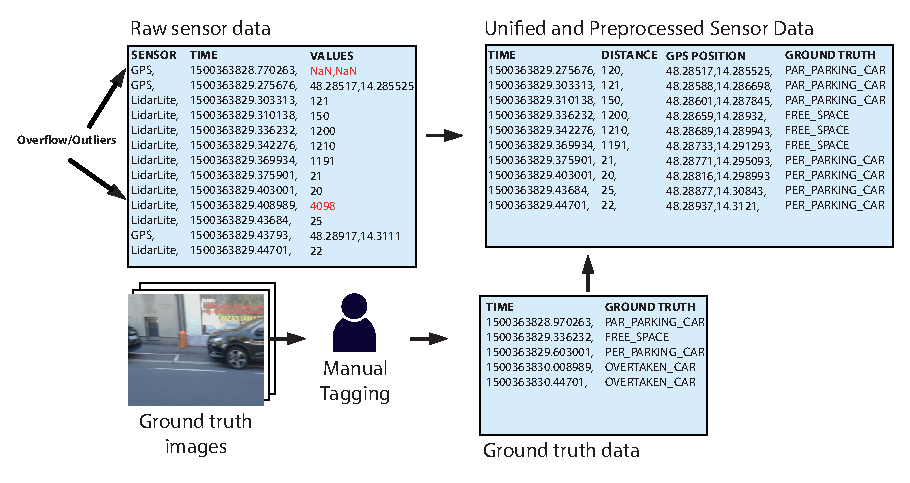
\includegraphics[width=\textwidth]{img/dataset-preprocessing.eps}
	\caption{\todo{todo} All sensor measurements are being merged to obtain a dataset where all samples are containing time, distance, location and ground truth information.}
	\label{fig:preprocessing_dataset}
\end{figure}





\section{Data Segmentation}
\label{sec:data_segmentation}

As the used distance sensor measures at a high frequency, it usually collects several distance measurements belonging to the same object. For example, if the sensing vehicle passes a parallel parked car (having a length of 4 meters) at a speed of 30 km/h it will collect approximately 24 measurements belonging to one passed car. It is necessary to group all measurements concerning this car; this is done by data segmentation of the preprocessed data.

There are several strategies how sensor data can be segmented, for example using sliding windows. However, such approaches will not work accurate enough in the case of street side parking detection, as the objects which should be segmented range from a few centimeters to a length of tens of meters. Therefore, a new strategy to segment the sensor data points is proposed. The used segmentation algorithm searches for high frequent changes in the distance signal and starts a new segment when the difference in distance between two consecutive measurements is above a certain segmentation threshold. Furthermore, if the timestamp of two measurements differ more than one second the start of a new segment will also be detected (this can be the case if the sensing vehicle was standing or driving at a very low speed and many measurements have been deleted in the preprocessing steps). 

To configure the threshold, experiments have been conducted with varying thresholds. The best threshold to detect the segmentation points in the distance sensor signal has been identified by manually reviewing the resulting segments for under- and over-segmentation. The resulting segmentation threshold is $1,05$ meters. This means that if two consecutive measures differ more than $1,05$ meters, the algorithm will assume that the sensor measurement belongs to a new object (e.g., a parking car or an overtaken car) and will detect a new segment.

\begin{figure}
	\centering
	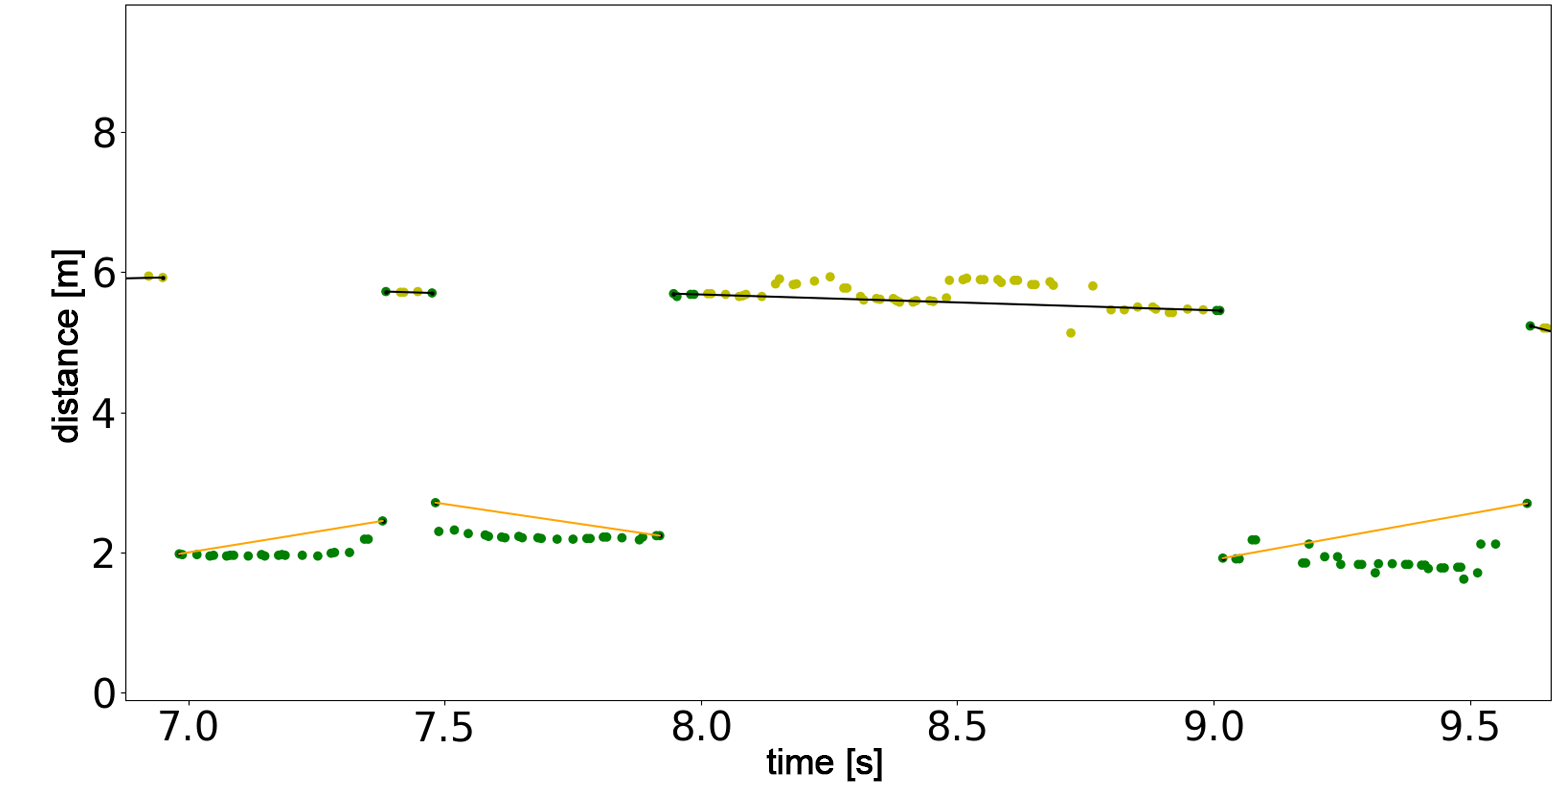
\includegraphics[width=0.95\textwidth]{img/segmentation_example.PNG}
	\caption{Result of the segmentation algorithm. Three parking cars (green dots and orange lines) and two free space segments (yellow dots and black lines) have been detected.}
	\label{fig:segmentation}
\end{figure}

Figure \ref{fig:segmentation} shows an example of the segmentation process. All points represent distance measurements. The green points represent measurements belonging to a parking car whereas the yellow points show free space measurements. The lines represent detected segments where belong to the same ground truth class. Black lines represent free space and orange lines represent a parking car. Thus, the segmentation shown in Figure \ref{fig:segmentation} has successfully detected three parking car- and two free space segments. 

Another challenge of the segmentation task is to estimate the ground truth classes of the segments. So far, only single sensor reading got a ground truth class assigned. However, as described earlier, each segment consists of multiple sensor measurements and it should be avoided that one segment consists of multiple different ground truth classes. This phenomenon is visible in Figure \ref{fig:segmentation} where both "Free space"-segments are overlapping with measurements marked as "Parking Car". To overcome this problem, the segments are tagged with the label of the majority of the sensor readings. This approach turned out to work well as in most cases only the first and last ground truth values are assigned wrong. 




\section{Feature Calculation}
\label{sec:feature_calculation}

To conduct machine learning experiments with common machine learning models, feature values for each segment have to be computed using the sensor measurements. These feature values serve as input values of the machine learning model to help classifying the corresponding segment to one of the available class labels. All computed features which were used are described below and a further analysis of the usefulness of the features for the classification tasks will be provided in Section \ref{sec:feature_analysis}.

\begin{description}

\item[Average distance to the sensing vehicle:] The average of the segment's distance sensor measurements to the closest object on the right side of the road in meters.

\item[Length:] The distance the sensing vehicle drove during sensing the segment in meters (the distance between the first and last GPS location).

\item[Duration:] The duration in seconds the sensing vehicle needed to sense the segment (the last time stamp - the first time stamp).

\item[Number of distance measurements:] The number of distance measurements assigned to the segment.

\item[Variance of the distance measurements:] The variance of all distance measurements belonging to the segment.

\item[Speed:] The speed of the sensing vehicle while sensing the segment in m/s.

\item[Acceleration:] The acceleration of the sensing vehicle while sensing the segment in $m/s^2$.

\item[Distance difference to the next/previous segment:] Difference of the average distance measurements to the next/previous segment in meters.

\end{description}







\section{Parking Space Maps}
\label{sec:parking_space_maps}

When sensing a city's parking availability situation parking space maps are of great importance. As already discussed, the machine learning models only classify road segments as "free spaces" (rather than "vacant parking spaces") which means that there are no parking cars. However, it is not clear whether parking is allowed. For example, a free space might just be a driveway or a bus station. Vacant parking spaces can be identified when their location is compared to a parking space map matching parking spaces there. 

The use of parking space maps will also possibly improve the performance of the classification task. If only segments in areas, where parking spaces are located, are used as training set, the overall data will be much more balanced (there will be less "free space" segments, but still almost the same amount of parking cars) and moreover the machine learning model will only be trained with relevant samples because only segments which are close to parking spaces have to be classified when generating a parking space availability map. Other segments do not add more information to such a map because it is known that in such areas it is not allowed to park.

%This section will describe the parking space maps which are available at the city authorities of Linz (Section \ref{sec:parking_space_map_linz}) as well as how a parking space map has been derived using clustering of parking spaces in the previously acquired dataset (Section \ref{sec:approximating_parking_space_maps}). Furthermore, the filtering of the dataset is discussed to obtain a more balanced dataset of only instances which are close to parking zones (Section \ref{sec:parking_space_maps_improve_classification}). Such an improved dataset should help to produce more accurate classification results on the machine learning experiments.



\subsection{Parking Space Map of Linz, Austria}
\label{sec:parking_space_map_linz}

As it is crucial to have accurate parking space maps, the goal was to obtain such maps for the area of the experiment. As a first try, the APIs of OpenStreetMap\footnote{\url{https://www.openstreetmap.org}} have been used to obtain map data of the city of Linz, Austria. 
%The maps of OpenStreetMap are created and maintained by independent communities which operate in their free time. 
Parking spaces are listed in the downloaded map data but unfortunately, only parking spaces of big parking lots (of shopping malls, etc.) are available but most of the city's road side parking spaces, which are being sensed in this work are not present. Therefore, the parking space maps of OpenStreetMap cannot be used due to insufficient data.

Another possibility to obtain a parking space map is to use data from city authorities in Linz. City authorities keep detailed digital maps of the streets as well as the road side parking spaces. However, the only format available are several DXF- or DWG-files, created using the program AutoCAD\footnote{\url{https://www.autodesk.eu/products/autocad/overview}}, which is commonly used for designing and drawing as well as for geographical applications. There exist libraries which can read all components of DXF-files and their attributes but unfortunately there are no geographical position data attached to the components and therefore the GPS location of all parking spaces is unknown. 
%Only an absolute coordinate from the drawing is available, but cannot be converted to a GPS location. 
This fact makes it impossible to use the parking space map in the park sensing prototype as the parking spaces of the map cannot be matched with the sensed segments obtained during the experiments.





%As it is crucial to have accurate parking space maps, the goal was to obtain such maps for the area of the experiment. As a first try, the APIs of OpenStreetMap\footnote{\url{https://www.openstreetmap.org}} have been used to obtain map data of the city of Linz, Austria. The maps of OpenStreetMap are created and maintained by independent communities which operate in their free time. Parking spaces are available in the downloaded map data but unfortunately, only parking spaces of big parking lots (of shopping malls, etc.) are available but most of the city's road side parking spaces, which are being sensed in this work are not present. Therefore, the parking space maps of OpenStreetMap cannot be used due to insufficient data.

%Another possibility to obtain a parking space map is to use data from city authorities in Linz. City authorities keep detailed digital maps of the streets as well as the road side parking spaces. However, the only format available are several DXF- or DWG-files, created using the program AutoCAD\footnote{\url{https://www.autodesk.eu/products/autocad/overview}}, which is commonly used for designing and drawing as well as for geographical applications. There exist libraries which can read all components of DXF-files and their attributes but unfortunately there are no geographical position data attached to the components and therefore the GPS location of all parking spaces is unknown. Only an absolute coordinate from the drawing is available, but cannot be converted to a GPS location. This fact makes it impossible to use the parking space map in the park sensing prototype as the parking spaces of the map cannot be matched with the sensed segments obtained during the experiments.



\subsection{Approximating Parking Space Maps}
\label{sec:approximating_parking_space_maps}

As parking space maps are unavailable in a sufficient quality from outside sources, an algorithm is introduced to derive a coarse parking space map from the dataset which was acquired during the test drives. The dataset contains the GPS positions of over 2.000 parking cars and most streets have been sensed several times. As of the limited amount of data, the goal is to create a coarse parking space map which contains areas where it is likely that vehicles park (parking zones). 

The proposed algorithm uses clustering to group parked cars to parking zones. The idea is that if there are several cars parking at the same location in several test drives then it is likely that there are parking spaces at that position. A DBSCAN\footnote{Density-Based Spatial Clustering of Applications with Noise - \url{http://scikit-learn.org/stable/modules/generated/sklearn.cluster.DBSCAN.html}} clustering algorithm (part of the scikit learn\footnote{\url{http://scikit-learn.org/}} python framework for machine learning) is being used to cluster the position of the parked cars. The DBSCAN algorithm searches for high density core samples and expands clusters from them. It takes the a similarity function which compares two data points and a minimum similarity as input parameters.

As similarity measure for the clustering algorithm a custom function has been implemented. Two parked cars are considered to be similar if the sensing car is driving in the same direction while sensing and if both cars are close to each other in terms of their GPS position. The first check is applied to ensure that both compared cars are parking at the same side of the street. Else it would be possible that two cars which park at the opposite side of the street are considered as belonging to the same "parking zone". If the first check is passed, the similarity function will compute the distance in meters between the GPS positions of both parked cars which are compared. The described similarity function is used by the DBSCAN clustering algorithm to identify core samples and to cluster multiple parking cars to parking zones. The maximum distance between two cars to be considered to be similar is set to eight meters. If two parking cars are further apart they are not considered to be able to be in the same parking zone. 
The result of the algorithm are clusters of parking cars which are considered as "parking zones" or "area where it is likely that cars are parking". To be able to determine if a specific GPS positions is in such a parking zone (needed later on for filtering), a bounding box is created for each cluster. Such a bounding box is created by taking the GPS position of the parking cars which are parking apart from each other the greatest distance. Around these two GPS positions a rectangle (the bounding box) is created by giving a ten meter error distance to all sides. The end result of the parking space map approximation is therefore a collection of parking zones, which are implemented as bounding boxes.

\begin{figure}
\centering
\def\arraystretch{1.2}

\begin{tabular}{ c }
	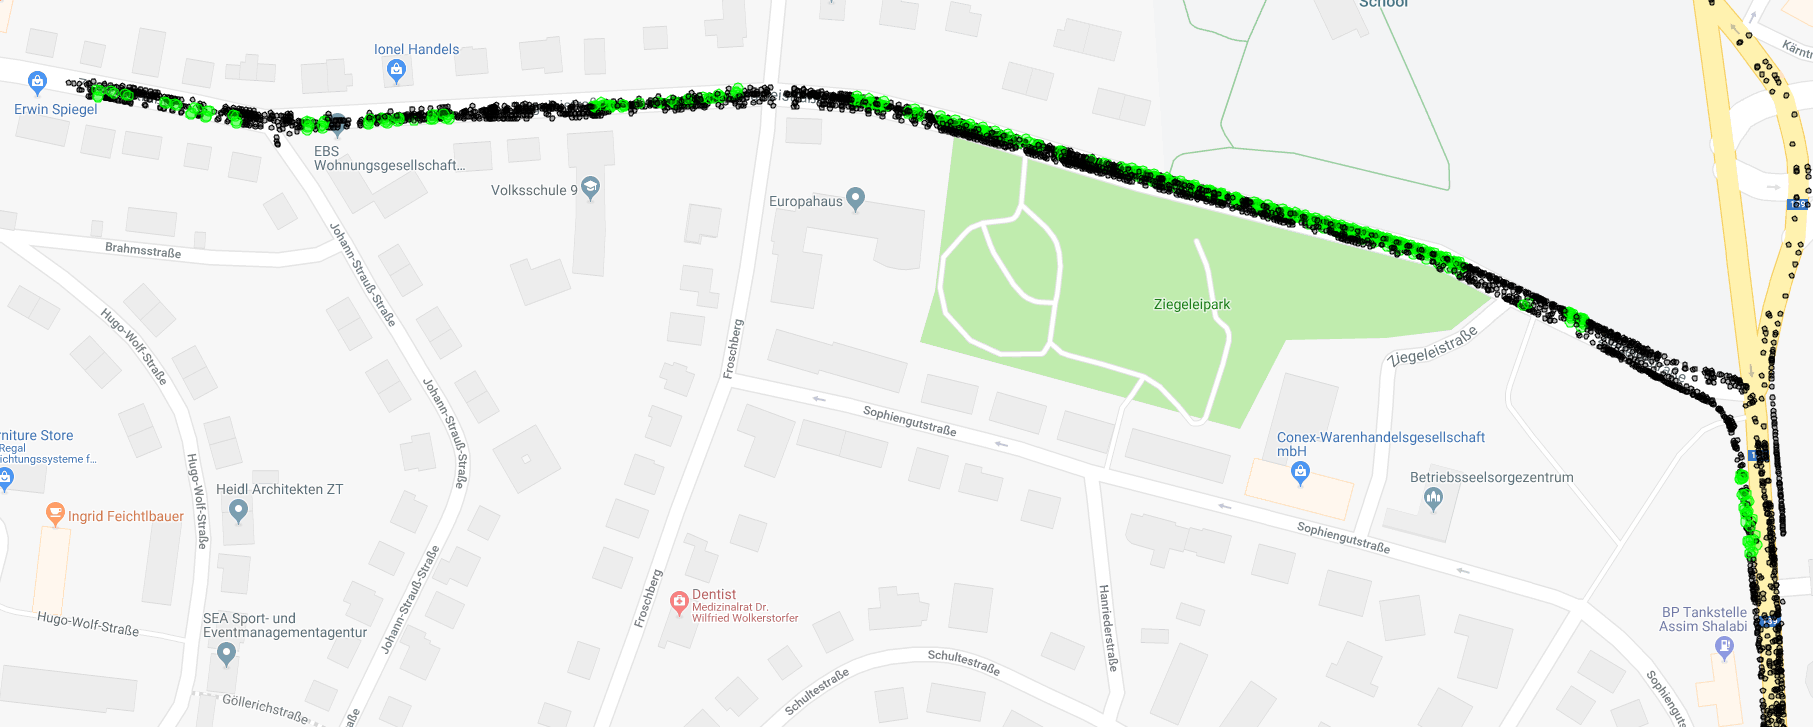
\includegraphics[width=0.9\textwidth]{img/parking_space_map_all_gps_2.PNG}
	\\
	(a) All GPS points
	\\
    \\
	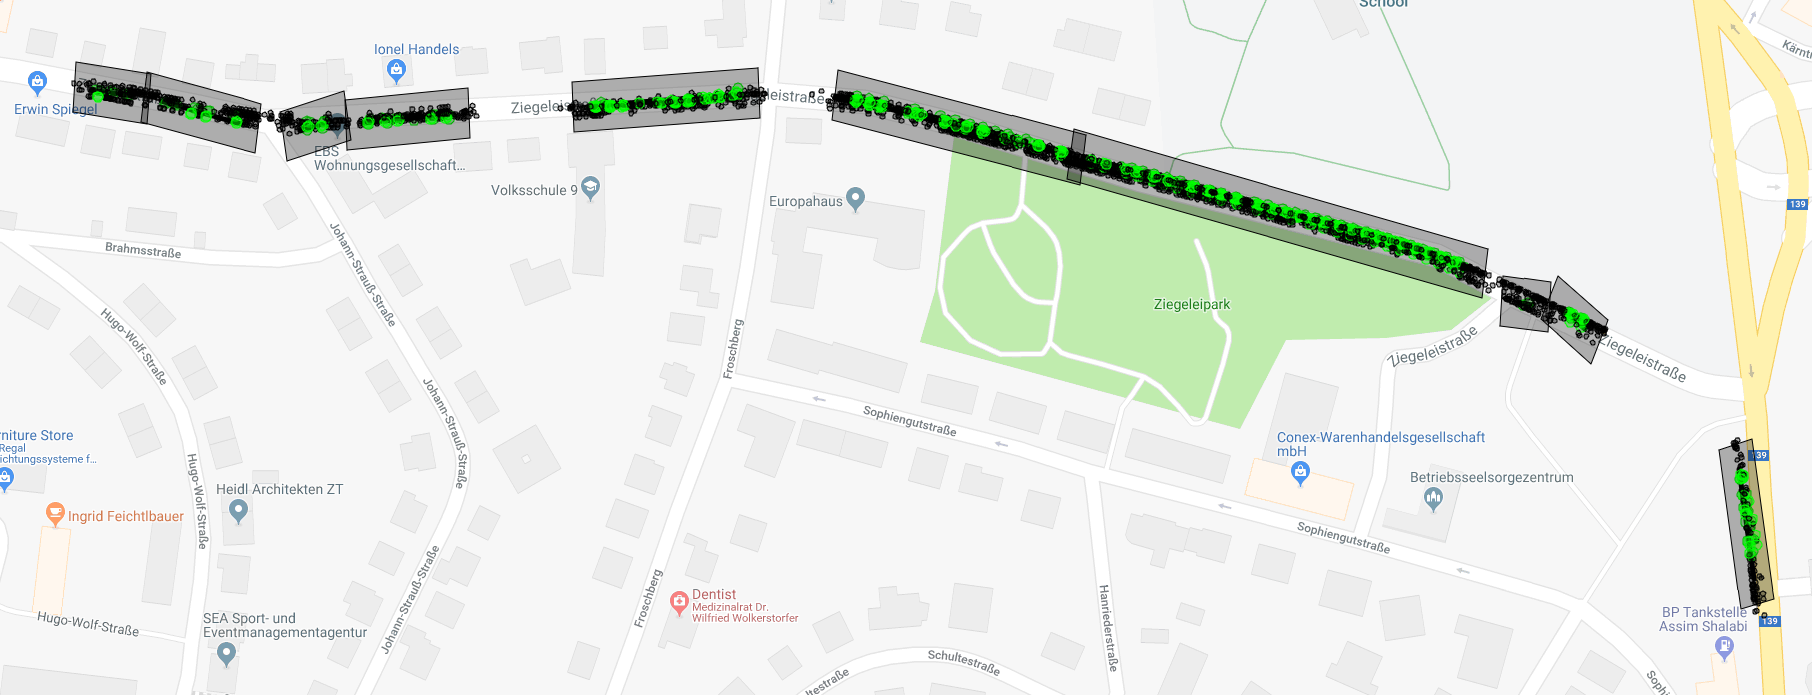
\includegraphics[width=0.9\textwidth]{img/parking_space_map_zones_2.PNG}
    \\
    (b) Detected parking zones
\end{tabular}

	\caption{Approximation of parking zones from the dataset: (a) showing all GPS points at the selected region while (b) showing the derived parking zones (clusters of parked cars).}
	\label{fig:parking_space_map}
\end{figure}

Figure \ref{fig:parking_space_map} shows two images of the same test region in Linz, Austria. In Figure \ref{fig:parking_space_map} (a) the GPS positions of all sensed segments, which are part of the dataset, while in Figure \ref{fig:parking_space_map} (b) only the GPS positions of segments which are in parking zones are shown. In both pictures green dots represent parking cars, while black dots show other segments. The semitransparent boxes which are shown in (b) show the clusters (parking zones) which were derived by the proposed algorithm. 
Only areas where there are lots of parking cars are extracted to be parking zones. In total 131 parking zones are derived from the whole dataset containing 97.2\% of all parking cars in the dataset. The remaining 62 parking cars are classified as noise by the clustering algorithm because there are no other parking cars in the dataset nearby. A larger dataset with more test drives during different times would be needed to get a more accurate parking space map and to reduce the parking cars which are classified as noise. However, because the most parking cars are contained in the derived parking zones, the parking space map can be used without a great loss to obtain a filtered and more balanced dataset as described in the following section.




\subsection{Using Parking Space Maps to improve Classification Results}
\label{sec:parking_space_maps_improve_classification}

As argued in Section \ref{sec:parking_space_maps}, it does not make sense to classify segments which are not close to parking zones. Such segments will not make a difference to the end result as it is known that at these positions parking is not possible (or legal) and there are not valid possible parking spaces. 
To improve the classification results, only segments which are close to parking zones will be used for training and for evaluating the machine learning models. The full dataset is further filtered by matching the GPS positions of the segments with the bounding boxes of the parking zones. All segments which are contained in at least one bounding box of a parking zone (and which are on the right side of the road) will remain in the dataset while all others are deleted. The full dataset as well as the filtered dataset and their differences are described in more detail in the following section.

%The remaining filtered dataset is much smaller than the original one. In total it consists of 8.591 segments, which are composed of 6.345 free spaces, 2.131 parking cars, 55 overtaking situations and 60 other parking vehicles. This filtered dataset is much more balanced than the original one, because almost all of the parking cars are still included while approximately half of the free spaces, which has been the dominating class, is deleted. Usually the more balanced dataset will lead to better values of precision and recall of the parking car class, but this has to be confirmed in the machine learning experiments. The results of the classification task using the parking space map filtered dataset can be found in Section \todo{ref}.








\section{Derived Datasets}
\label{sec:derived_dataset}

Two main datasets are being available for the use of machine learning experiments. The "full dataset" contains all segments which have been sensed during the test drives while "filtered dataset" has been filtered to only contain segments which are close to areas where parking spaces are located (described in the previous section). Both datasets are made up of samples with all calculated feature values (discussed in Section \ref{sec:feature_calculation}) and the corresponding class label.

Table \ref{table:dataset_comparison} shows a comparison of the number of instances per class for both datasets as well as the percentage of each class. One can clearly see that both datasets are highly imbalanced because in both cases the "free space" class is by far the dominating class with 83.6\% and 73.8\%, respectively. However, the filtered dataset contains only about half of the "free space" instances which are in the full dataset and thus the filtered dataset will probably lead to a better classification result as it is more balanced. Of course, this has to be proven by the machine learning experiments which will be covered in the following sections.

Another fact which can be observed is that the classes "overtaking situation" and "other parking vehicle" only have a really small percentage of the whole dataset size in both cases (both classes occur in the two datasets only in less than 2\% of the samples). For a good classification result it will probably be necessary to gain more data for these classes as with only such few instances the variety of the different instances will not be good enough for good classification results.
 
\begin{table}

%\resizebox{\textwidth}{!}{%
\centering
\bgroup
\def\arraystretch{1.4}
\begin{tabular}{| r || c | c |}
\hline
   & 
   \textbf{Full Dataset} & 
   \textbf{Filtered Dataset} \\
\hline
   \textbf{Free Space} & 
   11.811 (82.6\%) & 
   6.345 (73.8\%) \\
\hline
   \textbf{Parking Car} & 
   2.216 (15.5\%) & 
   2.131 (24.8\%) \\
\hline
   \textbf{Overtaking Situation} & 
   207 (1.4\%) & 
   55 (0.6\%) \\
\hline
   \textbf{Other Parking Vehicle}& 
   69 (0.5\%) & 
   60 (0.7\%) \\
\hline
\hline
   \textbf{Total}& 
   14.303 & 
   8.591 \\
\hline

\end{tabular}
\egroup
%}

\caption{Number and percentage of the segments per class in the two used datasets.}
\label{table:dataset_comparison}
\end{table}





\subsection{Feature Analysis}
\label{sec:feature_analysis}

The goal of each feature is to help identify the true class of a sample which should be classified. The feature analysis presented in this section should determine if all features are necessary and beneficial to this goal. Too many features maybe do not produce better results and also increase the learning time of all models. Using the tool Weka\footnote{\url{https://www.cs.waikato.ac.nz/ml/weka/}} two analytic approaches have been used, which show for each feature how useful it is for the classification tasks:

\begin{description}

\item[Information Gain Analysis:] Weka provides a tool called "InfoGainAttributeEval" which calculates the information gain (also known as entropy) of all the features for the classification task. The features which will contribute more to an accurate classification result will have a higher information gain than others. The resulting values are in the range of 0 to 1.

\item[Learner based Feature Analysis:] This approach tests several feature subsets on a real machine learning algorithm (a J48 decision tree is used) and identifies the best feature subset. Cross-validation is used for the experiment with different feature subsets and the result is a list of features which works best for the classification task using the tested machine learning algorithm. %The process is repeated with different training sets and counts how often the features are used in the different runs. If a feature is used in all runs it gets a value of 1 whereas if it is never used its value will be 0. So the higher the value is, the more the feature helps in the classification task.

\end{description}

Table \ref{table:feature_analysis} shows the results of the feature analysis process for the full and filtered datasets, respectively. The information gain shows that most features of the filtered dataset have a higher score, therefore probably the classification result will lead to a higher accuracy using the filtered dataset. Looking at the information gain of both dataset, six important features can be identified, having an information gain value over $0.1$ (average distance, different to previous and next segment, length, number of measures and duration). The remaining three features have a much lower information gain and therefore probably will not contribute as much to the classification result.

The learner based analysis confirms the results of the information gain analysis. All of the six most important features have been selected for the best feature subset in both datasets. It is also shown that the distance variance is not used in any case while the average speed and average acceleration are used in one case while being left out in the other.



\begin{table}


%\resizebox{\textwidth}{!}{%
\centering
\bgroup
\def\arraystretch{1.4}
\begin{tabular}{| r || c | c |}
\hline
   & 
   \textbf{} & 
   \textbf{Contained in best subset} \\
   & 
   \textbf{Information Gain} & 
   \textbf{(Learner based Analysis)} \\
   & 
   \textbf{Full/Filtered Dataset} & 
   \textbf{Full/Filtered Dataset} \\
\hline
  \textbf{Average distance} & 
   0.361 / 0.502 &
   yes / yes \\
\hline
\textbf{Diff to next} & 
   0.232 / 0.338 &
   yes / yes \\
\hline
\textbf{Diff to prev.} & 
   0.233 / 0.337 &
   yes / yes \\
\hline
\textbf{Length} & 
   0.223 / 0.290 &
   yes / yes \\
\hline
\textbf{Nr. of measures} & 
   0.178 / 0.235 &
   yes / yes \\
\hline
\textbf{Duration} & 
   0.175 / 0.234 &
   yes / yes \\
\hline
\textbf{Distance variance} & 
   0.055 / 0.067 &
   no / no \\
\hline
\textbf{Avg speed} & 
   0.019 / 0.022 &
   no / yes \\
\hline
\textbf{Avg acceleration} & 
   0.011 / 0.008 &
   yes / no \\
\hline


\end{tabular}
\egroup
%}

\caption{Feature analysis showing the information gain and learning based analysis results of all calculated features on the full and filtered dataset.}
\label{table:feature_analysis}
\end{table}






%Maybe 2-3 Graphics of the most important features (from Weka)









\section{Machine Learning Experiments}
\label{sec:machine_learning_experiments}

There are a lot of different machine learning approaches, which can be chosen from. All of them have their strengths and weaknesses and are applied in different scenarios. To find out which machine learning model works best for the parking space sensing scenario, experiments are being performed and the results are compared so that the best model can be identified. 
The overall goal of the experiments is to find the feature subset and the machine learning model which in combination produce the highest accuracy in classifying all segments. 
Especially the precision and recall values of the "parking car" class are of interest in our scenario, because detecting parking cars is crucial for creating accurate parking space availability maps.





\subsection{Tested Machine Learning Models}
\label{sec:machine_learning_models}

This section will discusses machine learning models which have been investigated on their performance on our datasets. Furthermore, also all parameters which could be set for the different machine learning models will be presented. The tested machine learning models are:


\paragraph{Naïve Bayes Classifier}

The Naïve Bayes classifier is based on the theory of conditional probabilities. For each class the probability is calculated, given the calculated features. Let $P(c|F)$ be the probability of a segment being a parked car $c$ given the features $F = {l, d}$ (length and distance). According to Bayes' rule the probability can be calculated as $P(c|F) = \frac{P(F|c) \times P(c)}{P(F)}$, where $P(F|c)$ is the probability of the features $F$ if the class is a parked car, $P(c)$ is the overall probability of a segment to be a parked car and $P(F)$ is the probability of the occurrence of the features $F$. Using Bayes' rule, probabilities of each class can be calculated given the related features. However, calculating the different probabilities in the equation is a non-trivial task and requires a lot of computing resources (especially if there are a lot of features). Therefore, Naïve Bayes introduces the assumption that all features in $F$ are independent to each other. Using this assumption the probabilities can be calculated with a much less complex equation: $P(c|F) = \frac{P(l|c) \times P(d|c) \times P(c)}{P(F)}$. $P(l|c)$ and $P(d|c)$ are the probabilities of the $length$- and $distance$-features given the class is a parking car. Both of these probabilities can be easily computed using the dataset. The independence-assumption greatly simplifies the solution, however, it also introduces error to the result as the features in most problems cannot be treated independently. In spite of its simplicity, the Naïve Bayes classifier can compete with more sophisticated classifiers in a lot of domains
 \cite{Hall2016_DataMining_ML}. 
%Its advantages are its fast learning and classification times, while its disadvantage is the over-simplification of the independence assumption which makes it inapplicable for many classification scenarios \cite{Hall2016_DataMining_ML}.



\paragraph{kNN Classifier}

A kNN classifier (k nearest neighbours) searches for the $k$ samples in the training set which are most similar to the sample which should be classified and then predicts the class which is contained in a majority of the found $k$ samples. To find similar samples, a similarity function has to be computed which calculates the similarity between the features of two samples. Such similarity functions are for example Euclidian distance, Manhattan distance or Chebyshev distance. For each classification, the classifier has to calculate the similarity to each sample in the training set and find the most similar $k$ samples. For big datasets this process can take a long time and another disadvantage is that the whole training set has to be saved for the classifier to work. Parameters for the kNN classifier are the number $k$ of nearest neighbours to search for and the similarity function \cite{Hall2016_DataMining_ML}.



\paragraph{Support Vector Machines (SVMs)}

\begin{figure}
	\centering
	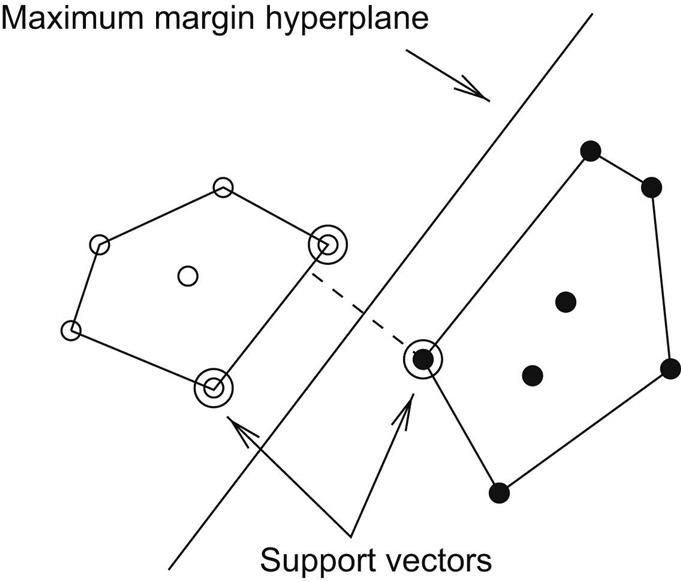
\includegraphics{img/max_hyperplane_weka_book.jpg}

	\caption{Maximum margin hyperplane of a support vector machine \cite{Hall2016_DataMining_ML}. \todo{kann ich die grafik aus dem buch verwenden oder soll ich sie nachzeichnen?}}
	\label{fig:max_hyperplane}
\end{figure}

Support vector machines try to find a linear separation between the samples of different classes in the training set in order to predict unknown samples. A hyperplane which maximizes the separation of different classes is being computed. In order to do so, the distance of the hyperplane to the closest samples, which are also called support vectors, is maximized. Figure \ref{fig:max_hyperplane} shows the so called maximum margin hyperplane as well as the support vectors which are needed to find it. However, in real world problems it is rarely the case that different classes can be separated using a linear hyperplane. To be able to find such an hyperplane, the feature space is transformed into a higher dimensional one using non-linear mappings. This process increases the chance of finding a hyperplane drastically. However, such transformations need a lot of computational performance and therefore usually kernel functions, such as a polynomial kernel, are used to speed up this process \cite{Hall2016_DataMining_ML}. 




\paragraph{Neural Networks}

A Neural Network (also called MultiLayerPerceptron in some frameworks) is a popular classification technique nowadays, because theoretically neural networks can learn every function possible given a large enough network and enough training time. Simple neural networks are composed of three layers: the input layer, a hidden layer and the output layer.





\paragraph{Decision Trees}

A powerful classification approach is a decision tree. Figure \ref{fig:decision_tree} shows an example of a decision tree which has been learned using the full dataset acquired in this thesis with the features length and distance. Each node divides the dataset into several sub-groups and at the leave nodes, the class with the majority of the samples is the classification result of the respective branch of the tree. The important task to learn a decision tree is to select the feature which should be used and where to split. This is done at each node by trying different features and values and finding the combination which maximizes certain measures, such as information gain or Gini impurity\footnote{Gini impurity represents how often a randomly chosen sample would be assigned into the wrong class if it was randomly labeled}. To overcome the risk of an over-fitting decision tree, the splitting process is stopped if there is a big majority or a single class at a node. This process is called pruning and can be controlled by a parameter called "confidence factor" \cite{Hall2016_DataMining_ML}.

\begin{figure}
	\centering
	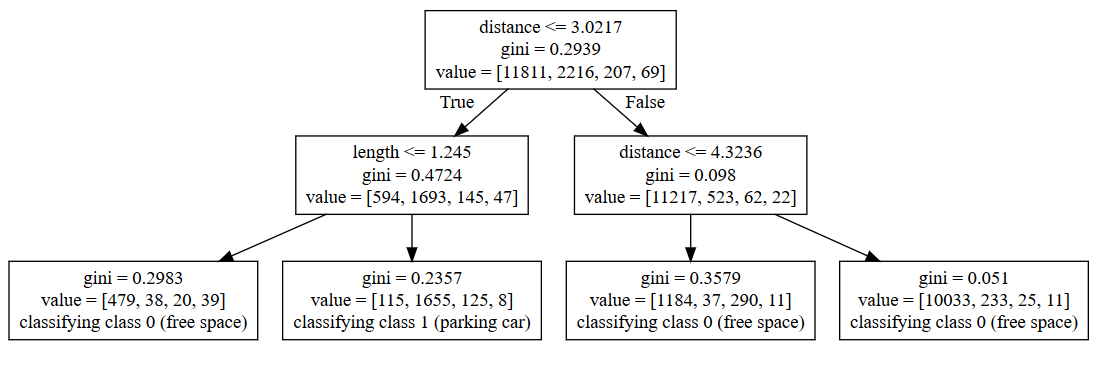
\includegraphics[width=\textwidth]{img/decision_tree2.PNG}

	\caption{Example of a decision tree with a depth of two, which has been trained with the full dataset and with the features length and distance.}
	\label{fig:decision_tree}
\end{figure}





\paragraph{Random Forest Classifier}

Decision trees can be rather unstable, meaning they can change their output drastically if their input is only altered slightly. To overcome this shortcoming, an ensemble technique, called "random forest" is introduced. A random forest classifier is made up of multiple different trees which have been learned using random subsets of features at each node of the trees during the training process. The outcoming trees are classifying using the input features and are then voting to determine the classification result of the random forest classifier. Random forests are usually creating more accurate predictions due to using many different decision trees which in conjunction produce better results as single decision trees. The most important parameters are the number of trees which should be generated, the random seed and the number of features per subset \cite{Hall2016_DataMining_ML}.













\subsection{Evaluation and Used Tools and Frameworks}

To be able to get reliable results for the performance of the different classifiers it is important to have a comparable evaluation method. The used method in this thesis is 10-fold cross validation. Using this technique, all samples of the dataset are split into 10 equally sized parts (folds). Then one fold is selected as test data while all the other folds are used as training data for the classifier. This process gets repeated 10 times, so that every fold has been used as test data exactly once and has been used for training all the other nine times. Cross validation ensures, that there is no sample in the test data which has been previously learned by the classifier in the training process. Moreover, it is important that every sample gets predicted once, so that the performance measures are realistic.

Another technique which helps to get better performance is to shuffle the dataset, before it is divided into folds for cross validation. The shuffling ensures that it is likely that only one of two consecutive segments is in the test data, while the other one is in the training data. This helps to have more diverse training data as consecutive segments usually are more alike than others. For example, usually perpendicular parking spaces are in the same area. Therefore, if the dataset gets shuffled the ratio between perpendicular parking spaces and other parking spaces will be approximately the same in the test- and training data.


%\subsection{Used Tools and Frameworks}

To conduct the machine learning experiments the dataset is processed using the Python programming language. Furthermore, the classifiers of the "Scikit learn" machine learning framework are used for the experiments and several different configurations of all of them are tested. Scikit learn is a framework for Python which offers all of the above discussed classifiers as well as tools to support the evaluation process (cross validation, shuffling, ...).






\section{Deep Learning}
\label{sec:deep_learning}

Deep learning gained a lot of attention in the last few years because of its raising classification accuracy results. For example, deep learning models became the first classifiers which could compete with humans on simple classification tasks. A deep learning network is a special form of a neural network with a possibly large amount of hidden layers between the input layer and the output layer. Furthermore, in many applications raw sensor measurements are used as input instead of pre-computed feature values, which are derived from the raw sensor values. In theory, a simple neural network containing only one hidden layer can derive any function given enough hidden elements and long enough training time. However, that does not mean that such a simple neural network will find a optimal solution and that it will find it in a finite amount of time. Adding more hidden layers (to get a deep neural network) can help to find a solution more easily and with less training time. 
Figure \ref{fig:densely_dl_network} shows an example of a deep learning network with several hidden layers which are densely-connected.

Due to the classification power, deep learning should also be tested for the use in classifying parking situations using our datasets. It should be investigated if deep learning can be used to do this kind of classification on raw sensor data and the results should be compared to classical machine learning algorithms (described in Section \ref{sec:machine_learning_models}) using pre-computed feature values.

%\subsection{Dataset for Deep Learning Experiments}

As input for the deep learning experiments a dataset containing all sensor measurements for each segment is needed. In a pre-processing step a dataset for the deep learning experiments is created which is made of a vector of sensor measurements for each segment. Each vector has a fixed size of 1024 sensor measurements (that will be enough for most segments). In most cases the segments have a much lower number of measurements. In these cases the measurements will be zero padded to the required size. If a segment has more than 1024 measurements, only the first 1024 will be used. This step is necessary to have a fixed length input for the experiments as the input size for all segments has to be equal. A vector represents the input layer of the neural network. 

\begin{figure}
	\centering
	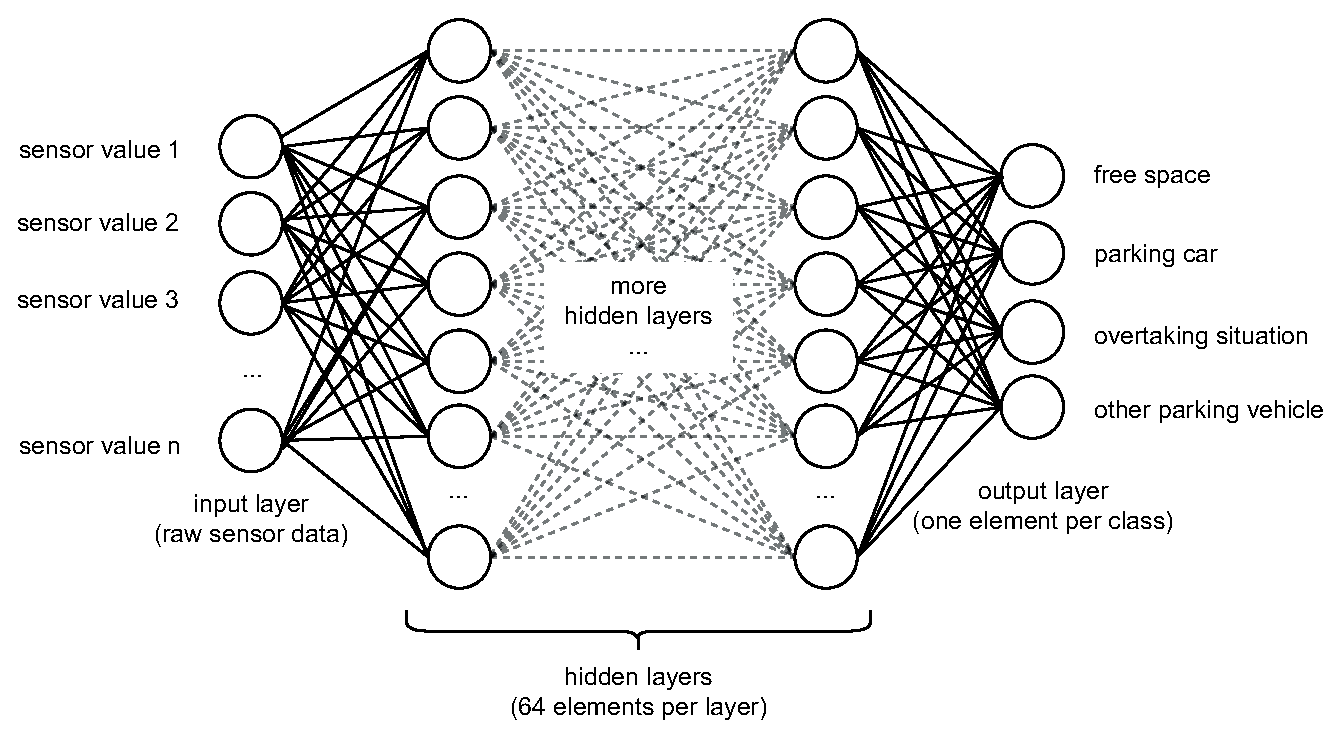
\includegraphics[width=\textwidth]{img/deep_learning_basic_model_2.eps}
	\caption{A basic deep learning network having sensor values as input and the probability of all classes as output values. All layers are densely connected with each other.}
	\label{fig:densely_dl_network}
\end{figure}





\subsection{Tested Deep Learning Models}

As baseline deep learning network a dense neural network with 5 hidden layers and 64 hidden elements per layer is used. This basic deep learning network should show how a densely-connected deep learning model performs on the raw sensor dataset. Figure \ref{fig:densely_dl_network} shows the illustration of the created deep learning network containing of an input layer with 1024 elements (one for each sensor value), 5 hidden layers containing 64 hidden elements per layer and four output elements which calculate the probability of each class for the given input. The class which gets predicted is the one with the greatest probability out of the four classes. 

In addition to the basic deep neural network, several known strategies should be tested to improve the performance of the deep learning approach. First of all, dropout between the layers should be tested. Dropout is a technique in deep learning to handle over-fitting of the neural network. If dropout with a prability $p$ is introduced between two layers, a connection between two elements is maintained only at a probability of $1-p$. The result is a more sparsely connected deep neural network which should be less prone to over-fitting. Dropout should be tested between several layers and with different values for the deletion-probability $p$.

Another popular technique to improve deep learning models is the use of convolution. Convolutional neural networks are especially popular for image classification. However, convolution can also be applied on the one-dimensional distance sensor data available in our dataset. Different configurations for the configuration of such a convolutional neural network should be tested and the performance should be compared to the other approaches.

\subsection{Tools and Frameworks used for developing Deep Neural Networks}

To implement the deep learning models, the programming language Python\footnote{\url{https://www.python.org/}} (version 3.6.4) is used as well as the Keras\footnote{\url{https://keras.io/}}- and the TensorFlow\footnote{\url{https://www.tensorflow.org/}} frameworks. Keras is used as a wrapper which is using the TensorFlow framework internally and helps to create easy to read representations of deep neural networks. TensorFlow is built for creating neural network models and especially for building deep learning models using a lot of pre-built components. 


Listing \ref{lst:deep_learning1} shows an example of a deep learning network which has been defined using the Keras framework. It defines a neural network with five hidden layers with each having 64 hidden elements using the ReLU activation function. Moreover, between every hidden layer there is a 20\% dropout of the connections between the hidden elements. To get a result, the output layer which consists of four elements is using the softmax activation function which calculates the probabilities for each class, therefore the output of the deep learning network is a vector with 4 numbers in the range of 0 to 1 adding up to 1. The listing furthermore shows the loss function (categorical crossentropy) as well as the optimizer (adam) and the used metric (accuracy).



\lstinputlisting[caption={Example of a densly-connected deep learning network containing 5 hidden layers with dropout defined with Keras}, language=Python, label={lst:deep_learning1}]{code/tensorflow_dense_neural_network.py}



